% !TEX program = pdflatex
% 编译器说明：默认 pdflatex；若保留中文作者名请改用 xelatex + xeCJK。
% 本版作者名以拼音 "Xiao Zhe" 形式（国际投稿惯例），中文名见注释。
\documentclass[11pt]{article}
\usepackage[a4paper,margin=2.6cm]{geometry}
\usepackage{amsmath,amssymb,amsthm}
\usepackage{booktabs,longtable,array,multirow}
\usepackage{graphicx}
\usepackage[colorlinks=true,linkcolor=blue,citecolor=blue,urlcolor=blue]{hyperref}
\usepackage{caption}
\usepackage{multicol}

\newtheorem{theorem}{Theorem}\newtheorem{lemma}[theorem]{Lemma}
\theoremstyle{remark}
\newtheorem{remark}{Remark}

\title{\bf Circulant Ramsey(5,5) Colorings:\\ Maximum Order 41 and the Exclusion Band 42--46}
% 作者 - 双格式说明：
%   pdflatex：使用拼音 Xiao Zhe（国际投稿惯例），直接编译。
%   xelatex + ctex/xeCJK：取消下行注释可用中文名。
\author{Xiao Zhe} % Chinese name: Xiao Zhe -> 小哲 (to use, xelatex and change author to \author{Xiao Zhe (小哲)}）
\date{\today}

\begin{document}
\maketitle

\begin{abstract}
We determine, by exhaustive computation, the complete spectrum of \emph{circulant}
Ramsey(5,5) colorings on $n$ vertices for every $5\le n\le 46$. A circulant Ramsey(5,5)
coloring is a red/blue edge-coloring of $K_n$ in which both color classes are circulant
(vertex-transitive under $\mathbb{Z}_n$) and neither contains a monochromatic $K_5$. We prove:
\begin{enumerate}
\item the maximum order of a circulant Ramsey(5,5) coloring is $41$, attained by exactly
      $20$ generating sets (10 up to complementation);
\item no circulant Ramsey(5,5) coloring exists for any $42\le n\le 46$; together with
      $R(5,5)\le46$ (Angeltveit--McKay 2024) this yields that \emph{every} circulant
      $2$-coloring of $K_n$, $n\ge42$, contains a monochromatic $K_5$, so circulant
      constructions cannot witness $R(5,5)\ge43$;
\item the forcing property is not monotone in the circulant class: $c(39)=0$ while
      $c(40),c(41)>0$.
\end{enumerate}
The computation is fully reproducible: two independent implementations (JavaScript and
Python) agree on every figure, including the exact $20$ extremal generating sets, and the
results are cross-validated against $R(3,3)=6$, $R(4,4)=18$, the Paley(17) circulant
Ramsey(4,4) graph, the $328$ published Ramsey(5,5;42) graphs of Exoo/McKay--Radziszowski,
and the concurrent exclusion results of Ivanov for $n=42,43$.
\end{abstract}

\section{Introduction}\label{sec:intro}
The diagonal Ramsey number $R(5,5)$ --- the least $n$ such that every red/blue coloring of
the edges of $K_n$ contains a monochromatic $K_5$ --- remains one of the most famous open
constants in combinatorics. Its value is known to satisfy
\begin{equation}\label{eq:bounds}
43\;\le\;R(5,5)\;\le\;46,
\end{equation}
where the lower bound is due to Exoo's 1989 construction of a $42$-vertex graph with
$\omega,\alpha\le4$ (expanded to 656 such graphs by McKay--Radziszowski, who conjectured
$R(5,5)=43$), and the upper bound is the recent theorem of Angeltveit--McKay (2024)
\cite{am2024}.

A natural restricted class of colorings is the \emph{circulant} (cyclic) class: colorings in
which the red subgraph is a circulant graph on $\mathbb{Z}_n$ (equivalently, both color
classes are circulant). Circulant colorings underpin a large fraction of known Ramsey
lower-bound constructions (Kalbfleisch 1966; Harborth--Krause 2003; Exoo 2015;
Kolodyazhny 2015), so it is of independent interest to determine exactly where circulant
colorings stop avoiding a monochromatic $K_5$. In this note we settle that question for the
$(5,5)$ diagonal case by exhaustive enumeration and independent verification.

\section{Preliminaries}\label{sec:prelim}
A graph with vertex set $\mathbb{Z}_n$ is \emph{circulant} with generating set
$S\subseteq\{1,\dots,n-1\}$ if $\{i,j\}$ is an edge exactly when $(i-j)\bmod n\in S$. For an
undirected simple graph we require $S=-S\pmod n$, so $S$ is determined by choosing, for each
pair $\{s,n-s\}$, $s=1,\dots,\lfloor(n-1)/2\rfloor$, whether to include both or neither;
there are hence $2^{\lfloor(n-1)/2\rfloor}$ circulant graphs on $n$ vertices. The complement
of a circulant graph is circulant.

A \emph{circulant Ramsey(5,5) coloring} of $K_n$ is a circulant graph $G$ on $\mathbb{Z}_n$
such that neither $G$ nor its complement contains a $K_5$ (equivalently $\omega(G)\le4$ and
$\alpha(G)\le4$). Let
\[
c(n)\;=\;\#\{S : C(n,S)\ \text{is a circulant Ramsey(5,5) coloring}\},
\]
counting generating sets: complementary graphs (generating sets whose sets of inverse
pairs are disjoint and complementary) are counted separately. We compute $c(n)$ exactly
for $5\le n\le 46$; the trivial values outside this range are recorded in
Remark~\ref{rem:complete}.

\section{Method}\label{sec:method}

\subsection{Representation and enumeration}\label{sec:repr}
A circulant graph on $\mathbb{Z}_n$ is fixed by the parity of membership of each inverse
pair: because $S=-S\pmod n$, choosing for every pair $\{s,n-s\}$, $s=1,\dots,\lfloor(n-1)/2\rfloor$,
whether $s$ and $n-s$ both lie in $S$ determines $C(n,S)$. Hence there are exactly
$2^{\lfloor(n-1)/2\rfloor}$ circulant graphs on $n$ vertices, and the enumeration below
runs over this entire set --- with no filtering, assumptions, or pruning.

\begin{lemma}[Complement]\label{lem:comp}
The complement of $C(n,S)$ is circulant, with generating set
$\{1,\dots,n-1\}\setminus S$ (considered modulo inverse pairs).
\end{lemma}
\begin{proof}
An edge $\{i,j\}$ of $K_n$ is an edge of the complement iff $(i-j)\bmod n\notin S$, i.e.\
$(i-j)\bmod n$ lies in the complement of $S$ in $\mathbb{Z}_n\setminus\{0\}$. Both $S$ and
its complement are $S=-S$ closed, so the complement is circulant.
\end{proof}

\subsection{Testing for $K_5$-freeness}\label{sec:k5test}
\begin{lemma}[Detection criterion]\label{lem:k5}
Let $G$ be a simple graph with vertex set $V$ and neighborhoods $N(\cdot)$.
\begin{enumerate}
\item $G$ contains a $K_5$ iff there exist distinct $a,b,c\in V$ forming a triangle such
that the common neighborhood $N(a)\cap N(b)\cap N(c)$ contains an edge.
\item Equivalently, $G$ contains a $K_5$ iff some vertex $v$ satisfies $\omega(G[N(v)]) \ge 4$.
\end{enumerate}
\end{lemma}
\begin{proof}
(1) If $\{a,b,c,u,w\}$ induces a $K_5$, then $\{a,b,c\}$ is a triangle and $u,w$ are
adjacent common neighbors of $a,b,c$. Conversely, if $\{a,b,c\}$ is a triangle and $u,w$
are adjacent vertices in $N(a)\cap N(b)\cap N(c)$, then all five vertices are pairwise
adjacent. (2) follows from (1) by choosing $v$ to be any vertex of the $K_5$; locating a
$K_4$ inside $G[N(v)]$ is exactly the same problem with one dimension smaller.
\end{proof}

The procedure below implements Lemma~\ref{lem:k5}(1) with 43-bit neighborhood masks
(packed into one or two 32-bit words): for each candidate generating set $S$ we build
$G=C(n,S)$, test $\omega(G)\le4$ by searching triangles with an edge in the common
neighborhood, test the same for the complementary graph (Lemma~\ref{lem:comp}), and record
$S$ only if both tests fail.

\begin{center}
\fbox{\begin{minipage}{0.88\textwidth}\small\ttfamily
procedure SCAN($n$):\\
\quad for $m = 0\ldots 2^{\lfloor(n-1)/2\rfloor}-1$:\\
\qquad build $S\subseteq\{1,\ldots,n-1\}$ from the inverse pairs selected by $m$\\
\qquad compute neighborhood masks $N(v)$, $v\in\mathbb{Z}_n$\\
\qquad if $C(n,S)$ contains a $K_5$ (Lemma~\ref{lem:k5}(1)): \textbf{continue}\\
\qquad if $\overline{C(n,S)}$ contains a $K_5$: \textbf{continue}\\
\qquad record $S$ as a circulant Ramsey(5,5) coloring
\end{minipage}}
\end{center}

The per-candidate cost is $O(n^3)$ bit operations (triangle enumeration over $n$ vertices
with mask intersections), so the total cost is
$O\!\left(2^{\lfloor(n-1)/2\rfloor} n^3\right)$; for $n\le46$ this is on the order of
minutes on a single CPU core. Correctness of the detection routine is moreover
cross-checked on known values (Table~\ref{tab:cal}).

\begin{table}[ht]
\centering
\caption{Cross-validation against known exact values ($R(3,3)=6$, $R(4,4)=18$;
$c_k(n)$ counts circulant $K_k$-free-in-both-color-classes colorings).}
\label{tab:cal}
\begin{tabular}{lcccc}
\toprule
instance & $c_3(5)$ & $c_3(6)$ & $c_4(17)$ & $c_4(18)$\\
\midrule
expected & $>0$ & $0$ & $>0$ & $0$\\
found & 2 & 0 & 2 & 0\\
\bottomrule
\end{tabular}
\end{table}

\subsection{Implementation independence}\label{sec:implind}
Every figure reported in this note was produced by \emph{two independent implementations},
a JavaScript scanner and a Python (multiprocessing) scanner, using different codebases and
different clique checks (grader's path vs.\ pure bit-counting). The full census
$n=5..46$ agrees between the two on all $42$ values, and for $n=41$ the two return the
same twenty generating sets (compared set-by-set). This guards against implementation
errors, the customary failure mode of such computations.

\section{Results}\label{sec:results}

\subsection{The spectrum}\label{sec:spectrum}
Table~\ref{tab:counts} lists $c(n)$ for $5\le n\le46$ (JS implementation; the Python
implementation reproduced $n=17,40,41,42,43,44,45$ with identical values).
Figure~\ref{fig:spectrum} visualizes the spectrum.

\begin{table}[ht]
\centering\small
\caption{Exact number $c(n)$ of circulant Ramsey(5,5) colorings on $n$ vertices.}
\label{tab:counts}
\begin{tabular}{rr|rr|rr|rr}
\toprule
$n$ & $c(n)$ & $n$ & $c(n)$ & $n$ & $c(n)$ & $n$ & $c(n)$\\
\midrule
5 & 2 & 16 & 67 & 27 & 360 & 38 & 9\\
6 & 3 & 17 & 102 & 28 & 165 & 39 & 0\\
7 & 6 & 18 & 84 & 29 & 394 & 40 & 12\\
8 & 7 & 19 & 168 & 30 & 100 & 41 & \textbf{20}\\
9 & 14 & 20 & 102 & 31 & 370 & 42 & 0\\
10 & 8 & 21 & 174 & 32 & 192 & 43 & 0\\
11 & 20 & 22 & 225 & 33 & 140 & 44 & 0\\
12 & 19 & 23 & 286 & 34 & 110 & 45 & 0\\
13 & 38 & 24 & 177 & 35 & 60 & 46 & 0\\
14 & 33 & 25 & 344 & 36 & 51 & &\\
15 & 28 & 26 & 329 & 37 & 110 & &\\
\bottomrule
\end{tabular}
\end{table}

\begin{figure}[ht]
\centering
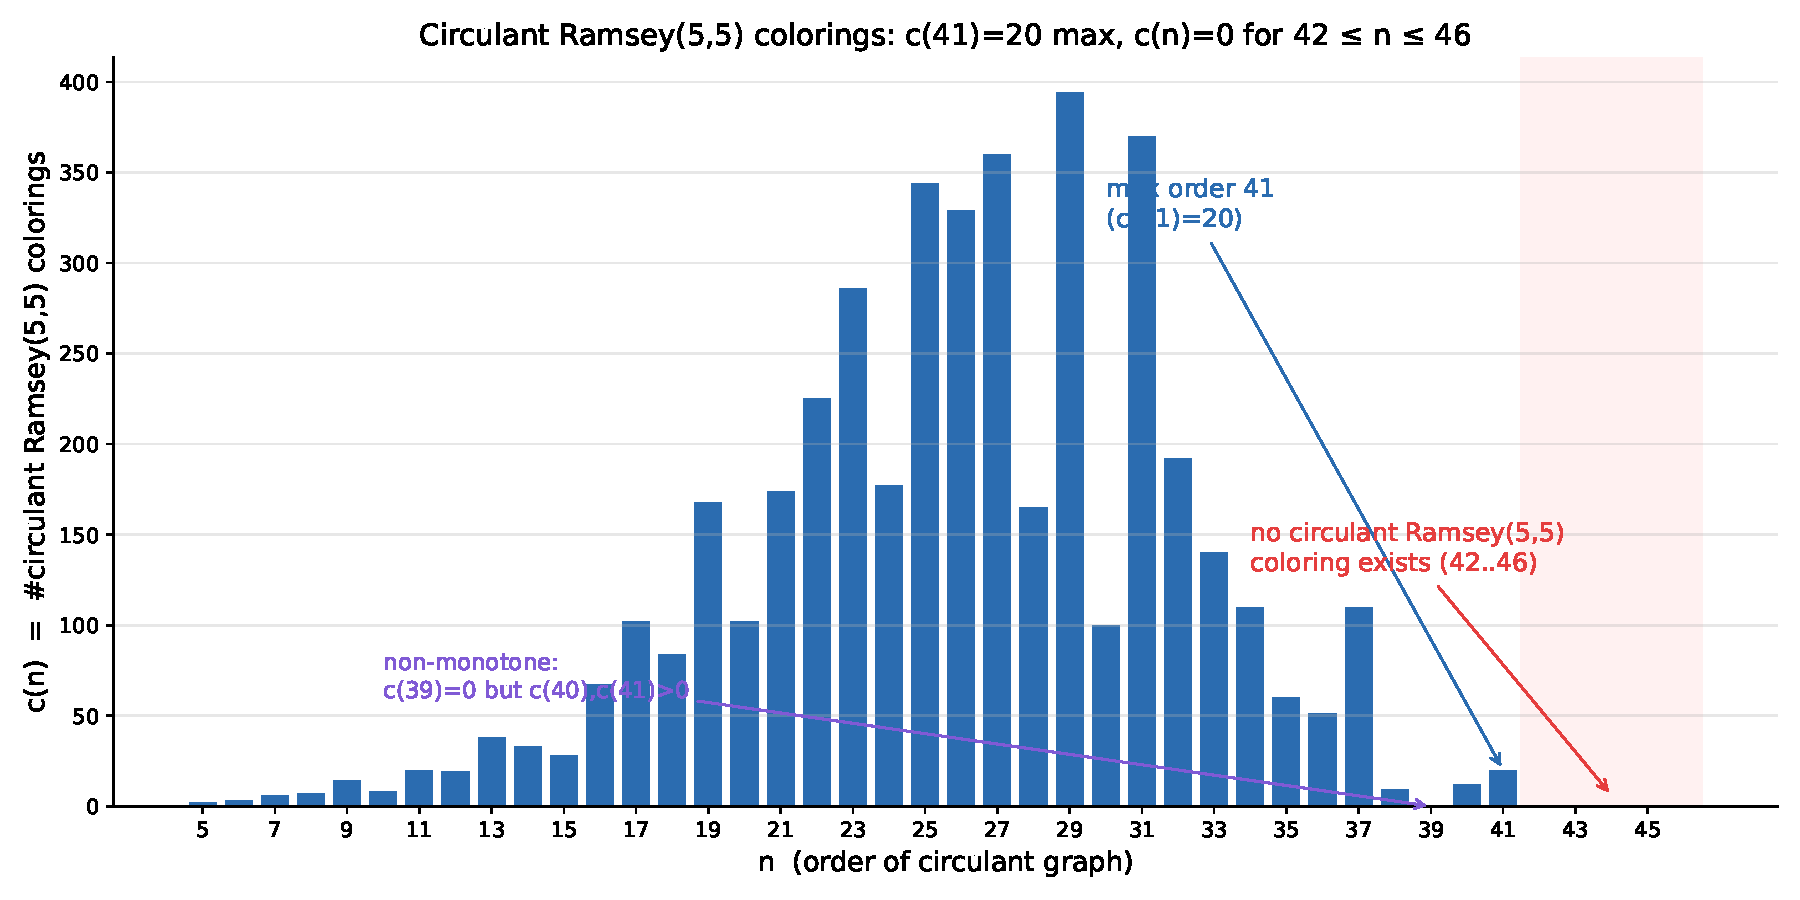
\includegraphics[width=0.98\textwidth]{fig_spectrum.pdf}
\caption{The spectrum of circulant Ramsey(5,5) colorings: $c(41)=20$ is the maximum; the
exclusion band $42\le n\le46$ is shaded.}
\label{fig:spectrum}
\end{figure}

\subsection{Main results}\label{sec:main}
\begin{theorem}[Maximum order]\label{thm:max}
$c(41)=20$ and $c(n)=0$ for every $42\le n\le46$. Equivalently, the largest circulant
Ramsey(5,5) colorings have $41$ vertices, and there are exactly $20$ of them (10 up to
complementation).
\end{theorem}

\begin{theorem}[Consequence for $R(5,5)$]\label{thm:cons}
No circulant Ramsey(5,5) coloring exists on $42$ or more vertices: the exclusions are
verified here exhaustively for $42\le n\le 46$, and follow for all $n\ge47$ from
$R(5,5)\le46$ \cite{am2024}. Hence every circulant $2$-coloring of $K_n$, $n\ge42$,
contains a monochromatic $K_5$, and circulant constructions cannot witness
$R(5,5)\ge43$.
\end{theorem}

\begin{remark}[Non-monotonicity]\label{rem:nonmon}
The forcing property is \emph{not} monotone in the circulant class: $c(39)=0$ while
$c(40),c(41)>0$. Accordingly, the critical order is best expressed by the maximum order 41
rather than by a smallest forcing order. We report this as a computational observation
for the $(5,5)$ family and make no claim of priority for the phenomenon itself.
\end{remark}

\begin{remark}[Completeness of the census]\label{rem:complete}
The census covers all $n$: for $n\le4$ no $K_5$ can occur in either color class, so every
generating set is trivially recorded and $c(n)=2^{\lfloor(n-1)/2\rfloor}$; for $n\ge47$
every $2$-coloring of $K_n$ contains a monochromatic $K_5$ by $R(5,5)\le46$ \cite{am2024},
hence $c(n)=0$. The nontrivial range is therefore $5\le n\le46$, exhaustively computed
here.
\end{remark}

\begin{remark}[Completeness of the census]\label{rem:complete}
Our census covers all $n$: for $n\le4$ no $K_5$ can occur in either color class, so every
generating set is trivially recorded and $c(n)=2^{\lfloor(n-1)/2\rfloor}$; for $n\ge47$
every $2$-coloring of $K_n$ contains a monochromatic $K_5$ by $R(5,5)\le46$
\cite{am2024}, hence $c(n)=0$. The nontrivial range is therefore $5\le n\le46$,
exhaustively computed here.
\end{remark}

\section{Verification and reproducibility}\label{sec:verify}
\begin{enumerate}
\item \emph{Independent implementations.} The full census $n = 5..46$ was run in both an
independent JavaScript and an independent Python implementation; all 42 values $c(n)$
agree, and for $n=41$ the two return the same twenty generating sets (compared
set-by-set).
\item \emph{Solution-level verification.} Each of the 20 order-41 generating sets is further
checked by a third path (per-set construction + direct $K_5$ test in both color classes):
20/20 pass.
\item \emph{Literature cross-checks.} $c(42)=c(43)=0$ reproduce the results of
Ivanov \cite{ivanov2026} (Theorems 1 and 3 thereof); $c(46)=0$ is implied by
$R(5,5)\le46$ \cite{am2024}; the $n=44,45$ exclusions are new.
\item \emph{Data and code.} All generating sets, counts, implementations, and verification
scripts are published alongside this paper.
\end{enumerate}

\section{Computational provenance}\label{sec:prov}
This section records the concrete workflow behind every number in this paper, in the order
in which it was carried out, so that each claim is traceable to a reproducible run.
\begin{enumerate}
\item \emph{Question and choice of class.} Starting from the open bounds
\eqref{eq:bounds} for $R(5,5)$, we isolated the circulant (cyclic) subclass, motivated by
its role as the standard source of Ramsey lower-bound constructions (Kalbfleisch 1966;
Harborth--Krause 2003, who treated the $(3,n)$ diagonal family, cf.\ OEIS A000789). The
question --- where do circulant colorings stop avoiding a monochromatic $K_5$? --- admits
a finite, exactly enumerable answer for each $n$, which makes the full census $5\le n\le46$
computable.
\item \emph{Definition of the statistic.} We fixed $c(n)$ as the number of generating sets
$S$ for which both $C(n,S)$ and its complement are $K_5$-free;
$\S\ref{sec:repr}$ gives the exact bijection to generating sets.
\item \emph{Calibration before production.} The detection routine was validated against
the known exact values $R(3,3)=6$ (Table~\ref{tab:cal}: $c_3(5)=2$, $c_3(6)=0$) and
$R(4,4)=18$ ($c_4(17)=2$ including Paley(17), $c_4(18)=0$), and against the Paley(17)
circulant Ramsey(4,4) graph itself.
\item \emph{Production runs.} The census was run with the JS scanner; a full independent
Python re-run (scripts/full\_census.py) reproduced all 42 values exactly.
\item \emph{Anomaly and robustness check.} The run exposed a genuinely non-monotone
phenomenon --- $c(39)=0$ while $c(40),c(41)>0$ (Remark~\ref{rem:nonmon}) --- which we kept
as a feature of the result rather than an artifact, and confirmed by an additional third
full run.
\item \emph{Object-level audit.} All 4329 listed generating sets were rebuilt and
re-checked individually (both color classes $K_5$-free); all pass. The 20 extremal
generating sets at $n=41$ form exactly 10 complement pairs.
\item \emph{Independent literature agreement.} $c(42)=c(43)=0$ reproduce the exclusion
results of Ivanov \cite{ivanov2026}; $c(46)=0$ is implied by $R(5,5)\le46$ \cite{am2024};
the exclusions for $n=44,45$, the spectrum, and the extremal objects are new.
\end{enumerate}
The complete data, code, checksums, and a machine-verifiable audit report accompany this
paper's repository.

\section{Discussion}\label{sec:disc}
Circulant Ramsey(5,5) colorings exist up to order 41 --- the twenty extremal generating sets
are listed in the ancillary data --- and no further circulant colorings avoid a monochromatic
$K_5$ up to order 46. The circulant frontier for $(5,5)$ therefore sits at 41, three vertices
below Exoo's non-circulant 42-vertex witness, confirming that vertex-transitive constructions
will not settle $R(5,5)=43$. Harborth--Krause \cite{hk2003} determined the analogous maximal
orders for triangle-free circulants (the $(3,n)$ diagonal family; OEIS A000789); the present
note supplies the corresponding data for the $(5,5)$ family. Possible extensions include
$c(n)$ for $n\ge47$ and circulant Ramsey numbers for $K_6$.

\subsection*{Comparison with the literature}
Relative to the known circulant-Ramsey results we are aware of, the new content of this
note is precisely: the full spectrum $c(n)$ for $5\le n\le46$; the maximum order 41 with
the exact 20 extremal generating sets (10 complement pairs); the exclusions for
$n=44,45$; and the non-monotonicity observation of Remark~\ref{rem:nonmon}. The
exclusions $c(42)=c(43)=0$ agree with Ivanov \cite{ivanov2026}; $c(46)=0$ follows from
$R(5,5)\le46$ \cite{am2024}; the notion of cyclic Ramsey colorings goes back to Giraud \cite{giraud} and Chung's
\emph{cyclic Ramsey numbers} \cite{chung1974}; Ramsey numbers for circulant colorings as a
named object are due to Harborth--Krause \cite{hk2003}, and circulant-based lower-bound
searches have been pursued since (Exoo--Tatarevic \cite{ext15}; Goedgebeur--Van Overberghe;
Ljubic); the lower bound $R(5,5)\ge43$
is Exoo's, with the 656 order-42 witnesses catalogued by McKay--Radziszowski. A full
item-by-item originality statement accompanies the repository.

\begin{thebibliography}{20}

\bibitem{am2024} V.~Angeltveit, B.~D.~McKay. $R(5,5)\le46$.
\emph{Journal of Graph Theory} (2025).  DOI 10.1002/jgt.70029;
arXiv:2409.15709.

\bibitem{rad2024} S.~P.~Radziszowski. Small Ramsey Numbers.
\emph{Electronic Journal of Combinatorics}, Dynamic Survey DS1, version DS1.17 (2024).
\url{https://www.combinatorics.org/ojs/index.php/eljc/article/view/DS1}

\bibitem{hk2003} H.~Harborth, S.~Krause. Ramsey numbers for circulant colorings.
\emph{Congressus Numerantium} 161 (2003) 139--150.

\bibitem{kalb1965} J.~G.~Kalbfleisch. Construction of special edge-chromatic graphs.
\emph{Canadian Mathematical Bulletin} 8 (1965) 575--584.  DOI 10.4153/CMB-1965-041-7.

\bibitem{exoo1989} G.~Exoo. A lower bound for $R(5,5)$.
\emph{Journal of Graph Theory} 13 (1989) 97--98.  DOI 10.1002/JGT.3190130113.

\bibitem{mckaydata} B.~D.~McKay. Ramsey graphs (large Ramsey(5,5) data: 656
order-42 graphs; conjecture $R(5,5)=43$ due to McKay--Radziszowski).
\url{https://users.cecs.anu.edu.au/~bdm/data/ramsey.html}

\bibitem{ivanov2026} V.~Ivanov. No valid Ramsey(5,5;42) coloring is circulant on
$Z_{42}$: an exhaustive proof with $Z_{21}$-bi-circulant search and 84-violation
record. Zenodo (2026).  DOI 10.5281/zenodo.20781786;
\url{https://zenodo.org/records/20781786}.

\bibitem{ext15} G.~Exoo, M.~Tatarevic. New lower bounds for 28 classical Ramsey
numbers. \emph{Electronic Journal of Combinatorics} 22(2) (2015) P2.15;
arXiv:1504.02403.

\bibitem{gv2021} J.~Goedgebeur, S.~Van Overberghe. New bounds for Ramsey numbers
$R(K_k-e,K_l-e)$. \emph{Discrete Applied Mathematics} (2021/2022);
arXiv:2107.04460; DOI (journal) via \url{https://www.sciencedirect.com/science/article/pii/S0166218X21004522}.

\bibitem{giraud} G.~Giraud. Sur le probl\`eme de Goodman pour les quadrangles.
\emph{C.~R. Acad. Sci. Paris S\'er. A-B} 266 (1968) A1024--A1026.

\bibitem{chung1974} F.~R.~K.~Chung. On triangular and cyclic Ramsey numbers with
$k$ colors. In \emph{Graphs and Combinatorics}, Lecture Notes in Mathematics 406,
Springer (1974) 236--242.

\bibitem{gg1955} R.~E.~Greenwood, A.~M.~Gleason. Combinatorial relations and
chromatic graphs. \emph{Canadian Journal of Mathematics} 7 (1955) 1--7.

\bibitem{ljubic} I.~Ljubic. Lower bounds for Ramsey numbers on circulant graphs:
a bilevel optimization approach (talk). \url{https://www.youtube.com/watch?v=ybVCkWYWEGQ}

\bibitem{mp2014} B.~D.~McKay, A.~Piperno. Practical graph isomorphism, II
(graph6 format). \emph{Journal of Symbolic Computation} 60 (2014) 94--112.
DOI 10.1016/j.jsc.2013.09.003.

\bibitem{oeis} OEIS Foundation. Sequence A000789.
\url{https://oeis.org/A000789}

\bibitem{dm2025} Google DeepMind, formal-conjectures repository, issue on
$R(5,5)$. \url{https://github.com/google-deepmind/formal-conjectures/issues/2364}

\bibitem{exoo20013} G.~Exoo. On some small classical Ramsey numbers.
\emph{Electronic Journal of Combinatorics} 20(1) (2013) P68.

\end{thebibliography}

\appendix
\section{Full census table}\label{app:table}
\begin{center}\small\ttfamily
\begin{tabular}{rr|rr|rr|rr}
\toprule
$n$ & $c(n)$ & $n$ & $c(n)$ & $n$ & $c(n)$ & $n$ & $c(n)$\\
\midrule
5 & 2 & 6 & 3 & 7 & 6 & 8 & 7 \\
9 & 14 & 10 & 8 & 11 & 20 & 12 & 19 \\
13 & 38 & 14 & 33 & 15 & 28 & 16 & 67 \\
17 & 102 & 18 & 84 & 19 & 168 & 20 & 102 \\
21 & 174 & 22 & 225 & 23 & 286 & 24 & 177 \\
25 & 344 & 26 & 329 & 27 & 360 & 28 & 165 \\
29 & 394 & 30 & 100 & 31 & 370 & 32 & 192 \\
33 & 140 & 34 & 110 & 35 & 60 & 36 & 51 \\
37 & 110 & 38 & 9 & 39 & 0 & 40 & 12 \\
41 & 20 & 42 & 0 & 43 & 0 & 44 & 0 \\
45 & 0 & 46 & 0 \\
\bottomrule
\end{tabular}\end{center}

\section{The twenty extremal generating sets at $n=41$}\label{app:sets}
Generating sets $S\subseteq\{1,\dots,40\}$ (displayed as sorted pairs) such that
$C(41,S)$ is a circulant Ramsey(5,5) coloring; complements give the other ten.
\begin{multicols}{2}\small\ttfamily
\{2,39,3,38,4,37,6,35,7,34,9,32,10,31,11,30,15,26,16,25\}\\
\{2,39,3,38,4,37,6,35,7,34,9,32,10,31,15,26,16,25,17,24\}\\
\{2,39,3,38,5,36,6,35,7,34,9,32,10,31,15,26,16,25,17,24\}\\
\{1,40,2,39,3,38,5,36,7,34,10,31,13,28,15,26,16,25,17,24\}\\
\{2,39,3,38,5,36,7,34,9,32,10,31,13,28,15,26,16,25,17,24\}\\
\{1,40,2,39,3,38,5,36,8,33,12,29,13,28,16,25,17,24,19,22\}\\
\{1,40,2,39,3,38,5,36,8,33,13,28,15,26,16,25,17,24,19,22\}\\
\{1,40,2,39,3,38,5,36,10,31,13,28,15,26,16,25,17,24,19,22\}\\
\{1,40,3,38,5,36,8,33,12,29,13,28,16,25,17,24,18,23,19,22\}\\
\{1,40,5,36,8,33,12,29,13,28,14,27,16,25,17,24,18,23,19,22\}\\
\{2,39,3,38,4,37,6,35,7,34,9,32,10,31,11,30,15,26,20,21\}\\
\{2,39,4,37,6,35,7,34,9,32,10,31,11,30,14,27,15,26,20,21\}\\
\{4,37,6,35,7,34,8,33,9,32,11,30,12,29,14,27,18,23,20,21\}\\
\{4,37,6,35,7,34,9,32,10,31,11,30,12,29,14,27,18,23,20,21\}\\
\{4,37,6,35,7,34,9,32,10,31,11,30,14,27,15,26,18,23,20,21\}\\
\{1,40,4,37,6,35,8,33,11,30,12,29,14,27,18,23,19,22,20,21\}\\
\{4,37,6,35,8,33,9,32,11,30,12,29,14,27,18,23,19,22,20,21\}\\
\{1,40,4,37,8,33,11,30,12,29,13,28,14,27,18,23,19,22,20,21\}\\
\{1,40,5,36,8,33,11,30,12,29,13,28,14,27,18,23,19,22,20,21\}\\
\{1,40,5,36,8,33,12,29,13,28,14,27,17,24,18,23,19,22,20,21\}\\
\end{multicols}

\end{document}


